\documentclass{article}
\usepackage{graphicx}
\graphicspath{{../images/}}

\begin{document}
\newcommand{\plugin}[1]{\texttt{#1}}
\section{Cholecystitis Case Study}
\label{sec:Cholecystitis}
\subsection{Cholecystitis Pathway Variants}
This section shows the cholecystitis pathway variant plot auto-generated by ProM. Cholecystitis pathway variants are analyzed without activities from the `antibiotics' sub-process and the `monitoring labs' sub-process (see Fig.~\ref{fig:cholecystitispathwaymodel} for the activities from the two sub-processes). Clinicians confirmed that these sub-processes are standard monitoring and maintenance systems while the patient is waiting for further diagnosis. Only analyzing activities from the primary cholecystitis pathway significantly reduces the level of clinical variation between patient traces.

The cholecystitis pathway model consists of 10 pathway variants. The 10 pathway variants of the cholecystitis pathway model are shown in Fig.~\ref{fig:cholecystitispathwayvariants}, and the number of patient traces that follow each pathway variant are listed in Table \ref{table:cholecystitisvarianttable}. Pathway variants from Fig.~\ref{fig:cholecystitispathwayvariants} are sorted from the most common pathway (index 0) to the least common pathway (index 9). The most common pathway variant (index 0) consists of anesthesia, surgery, and surgical pathology lab. The second pathway variant (index 1) includes surgery without anesthesia because of faulty clinical data.

\begin{figure}[t]
\hspace{-2cm}
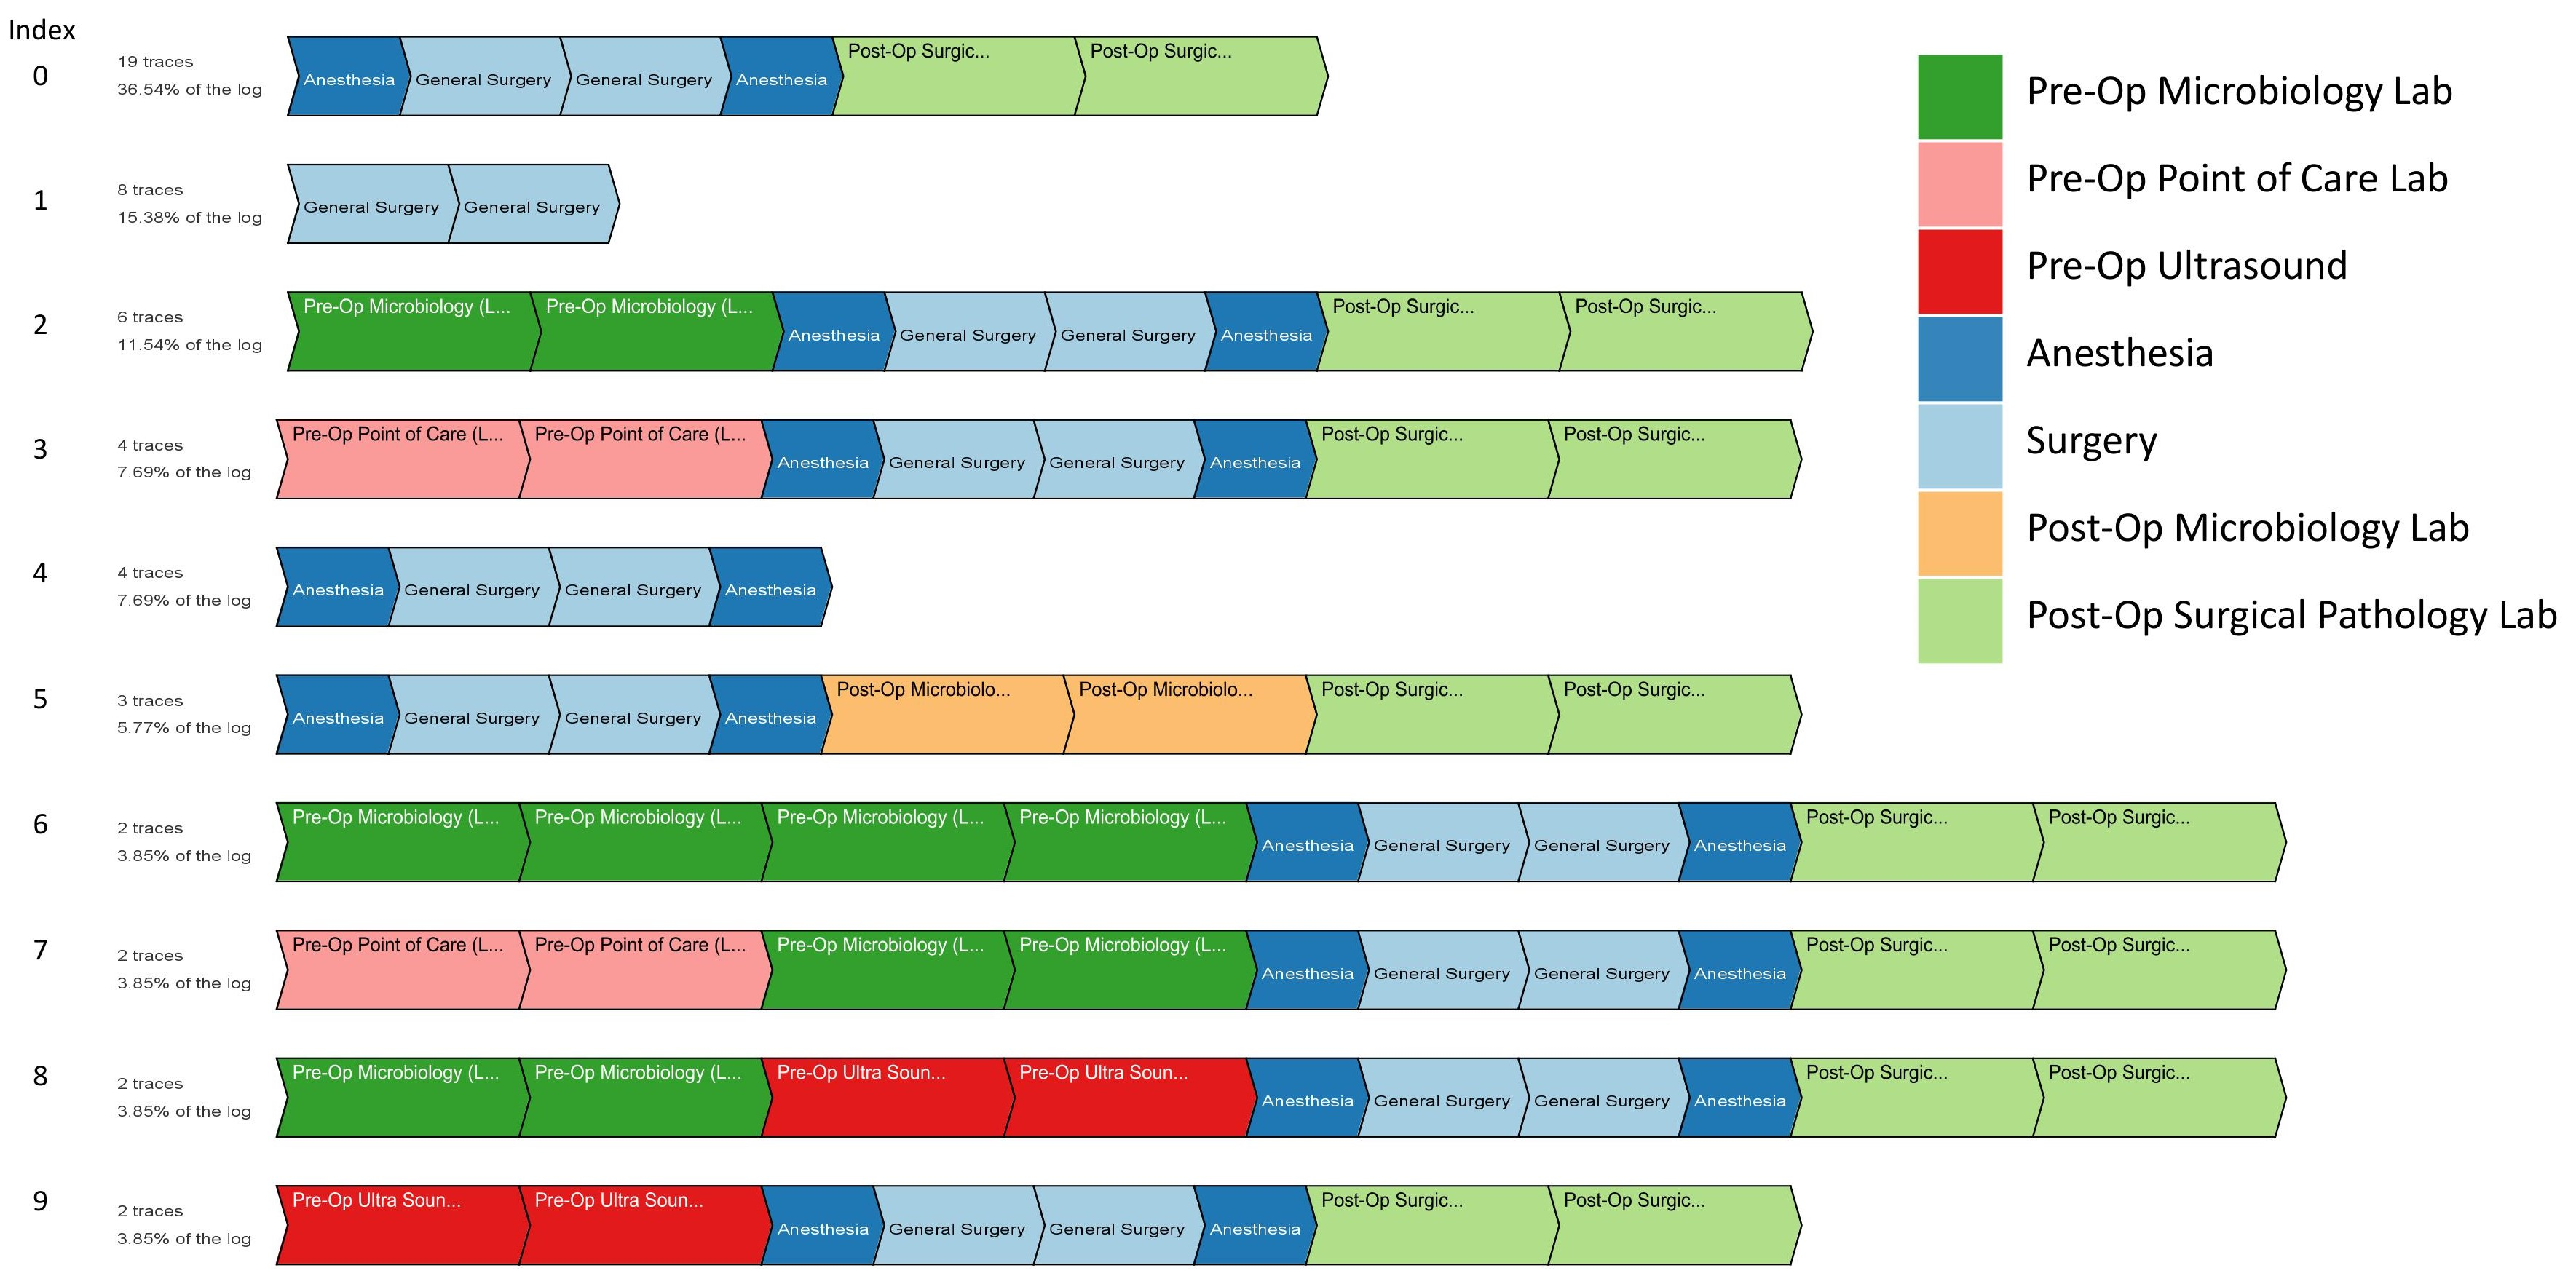
\includegraphics[width=1.5\textwidth]{cholecystitis_variant_index_anes.jpg}
\caption{Cholecystitis pathway variant plot auto-generated by ProM's plugin \plugin{Explore Event Log}. For the purpose of readability the legend was added and the statistics on the left are repeated in Tab.~\ref{table:cholecystitisvarianttable}.
The top three variants account for approximately 63\% of the patient traces.}
\label{fig:cholecystitispathwayvariants}
\end{figure}

\begin{table}[t]
\centering
\caption{Statistics of cholecystitis patient traces shown in Fig.~\ref{fig:cholecystitispathwayvariants}.}
\label{table:cholecystitisvarianttable}
\begin{tabular}{llllll}
  \hline
  \hline
Variant &     0  &     1  &     2  &     3  &    4\\
\hline
Patients   &    19 &     8 &     6 &     4 &    4\\
  Percentage &  36.54\% &  15.38\% &  11.54\% &  7.69\% &  7.69\%\\
  \hline
  \hline
Variant &     5  &    6  &    7  &    8 &    9\\
\hline
Patients   &   3 &     2 &     2 &     2 &     2 \\
Percentage &  5.77\% &  3.85\% &  3.85\% &  3.85\% &  3.85\% \\
  \hline
  \hline
\end{tabular}
\end{table}

\subsection{Cholecystitis Pathway Model}
The cholecystitis pathway model visualized by \texttt{`Inductive Visual Miner'} incorporates activities from the `antibiotics' sub-process and the `monitoring labs' sub-process. A breakdown of the cholecystitis pathway model into one primary pathway and two concurrent sub-processes is shown in Fig.~\ref{fig:cholecystitispathwaymodel}, and the model notations are summarized in Table \ref{table:notation}. The first pathway model in Fig.~\ref{fig:cholecystitispathwaymodel} is the primary pathway, followed by the `antibiotics’ sub-process and the `monitoring labs’ sub-process. Patient traces can execute any combination of the two sub-processes concurrently with the primary pathway. The eight patient traces that follow the second pathway variant (index 1) do not conform to this pathway model because of faulty clinical data. Based on this model, pre-operation haematology and chemistry labs tend to span the entire pre-operation process, while pre-operation antibiotics are taken closer to surgery.

\begin{figure}[t]
\centering
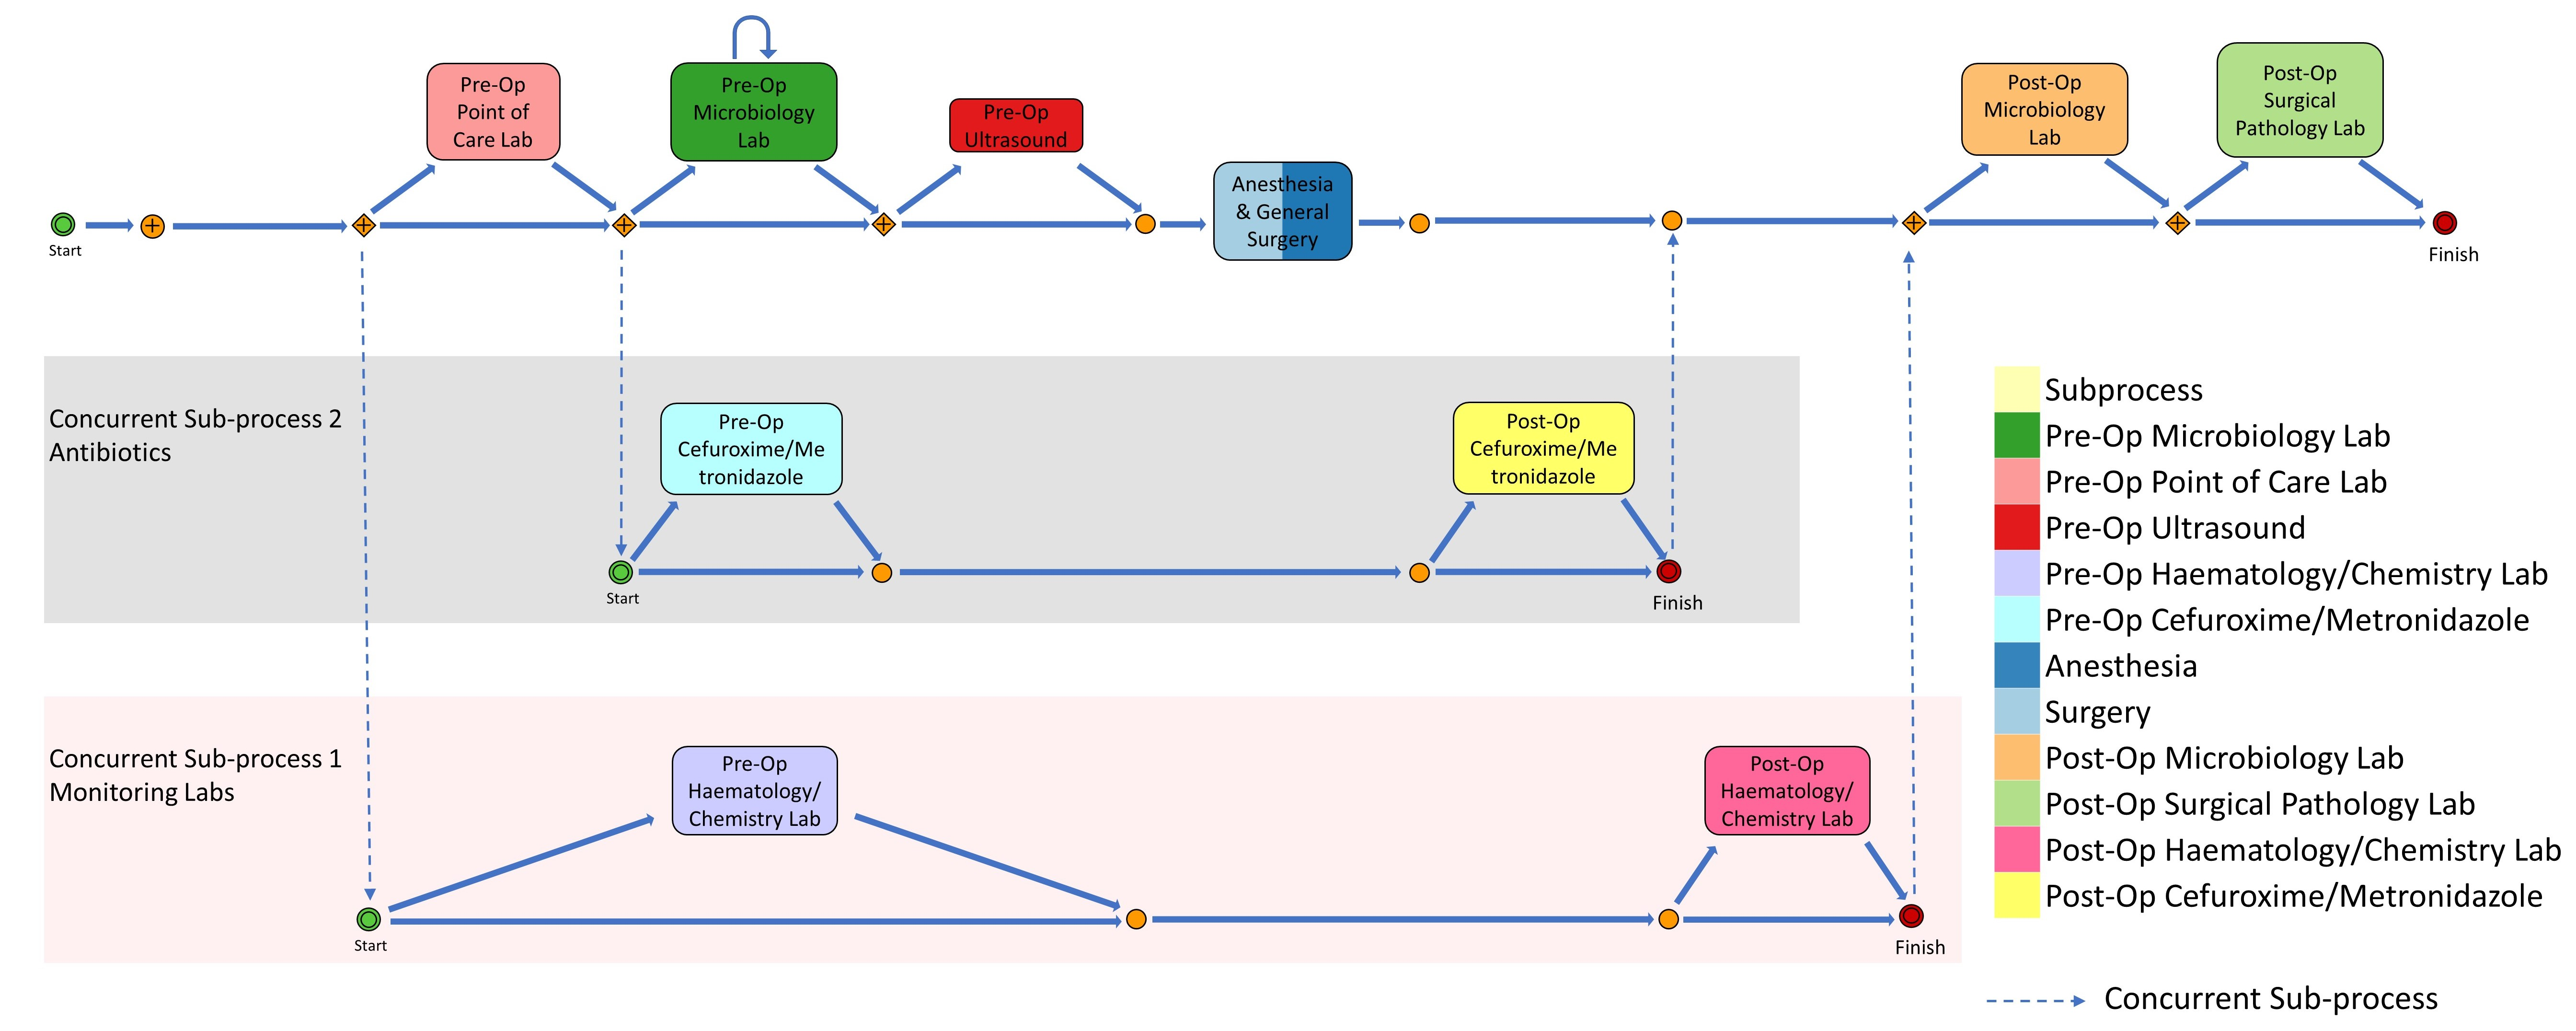
\includegraphics[width=18cm,angle=270]{communicative_cholecystitis_process_models_anes.jpg}
\caption{Cholecystitis pathway model using nomenclature of Tab.~\ref{table:notation}. The model is broken down into one primary pathway and two sub-processes.}
\label{fig:cholecystitispathwaymodel}
\end{figure}


\begin{table}[t]
\centering
\caption{Definitions of new pathway model notations \cite{PDHpathways}.\label{table:notation}}
\begin{tabular}{ l c l }
 \hline
 \hline
 Notation & Symbol & Definition \\ 
 \hline
 Orange Diamond 
 &
%\raisebox{-\totalheight}{\includegraphics[width=0.3\textwidth, height=60mm]{images/myLboro.png}}
 \raisebox{-3pt}{
\includegraphics[width=0.5cm]{decision_node.png}}
 & Decision Point, indicating exclusive choice \\ 
 \hline
 Orange Connector 
 & 
 \raisebox{-3pt}{
\includegraphics[width=0.5cm]{connection_node.png}}
 & Pathway Connection Point \\
 \hline
 Green Connector 
 & 
 \raisebox{-3pt}{
\includegraphics[width=0.5cm]{start_node.png}}
 & Starting Point \\
 \hline
 Red Connector 
 & 
 \raisebox{-3pt}{
\includegraphics[width=0.5cm]{finish_node.png}} 
 & Finishing Point \\
 \hline
 \hline
\end{tabular}
\end{table}

\bibliographystyle{unsrt}
\bibliography{/Users/obi/01-Exocortex/research/doc/bibliography/my_publications}

\end{document}